\chapter{Fundamentação Teórica}
\label{chap:fundteorica}
Nessa parte será apresentados conceitos para melhor entendimento deste trabalho e da modelação utilizada. 
A seção \ref{chap:grafos} elucida o que são grafos e o capítulo \ref{chap:redecomplexa} explica a variação de grafo utilizado para modelar o problema proposto. Depois na seção \ref{chap:lol} é esclarecido o ambiente que será abstraído, explicando algumas regras básicas do jogo.
\section{Grafos}
\label{chap:grafos}

Quando descrevemos uma situação utilizando pontos e ligações entre algum desses pontos, como o exemplo os pontos sendo pessoas e as ligações entre as pessoas sendo as amizades feitas, a abstração matemática desse tipo dá lugar ao conceito de grafo \cite{Lucchesi1979}.

Segundo \citet{Viana2007} "Um grafo \(G(V, E)\) pode ser definido como um conjunto de vértices \(V\), e um conjunto de conexões \(E\) " e ele continua: "Cada elemento do conjunto \(E\), associa dois elementos do conjunto \(V\), assim, se \((u,v) \in E\), então existe uma conexão entre os vértices u e o vértice v .". Sendo eles classificados como vizinhos ou adjacente \cite{grafosucinto}.

Nas próximas sub-seções será descrito características básicas de grafo que são essenciais para o entendimento do trabalho aqui descrito. Na seção \ref{chap:redecomplexa} será explicado sobre a modelação do mundo real em forma de grafos e como esse grafo especial é chamado.


\subsection{Binário e Não-binário}
Os grafos também podem ser classificados como binários e não-binários, sendo os binários suas arestas representadas por 1 ( se existem ) ou 0 ( se não existem ) e os não-binários quando existe um conjunto \(W\) onde informa a intensidade da interação de uma aresta entre dois vértices  \cite{Viana2007}.
Na Figura \ref{fig:grafo-exemplobinario} temos um grafo binário onde se \((u,v) \in E\) então ela está representada no grafo, já na Figura \ref{fig:grafo-exemplonaobinario} além da existência da conexão entre os vértices, está representado o conjunto \(W\) informando o peso ou aresta daquela aresta.

\begin{figure}[!h] \centering
	\centering
	\caption{Exemplo de grafos.}
	\subfloat[Grafo binário com quatro vértices e quatro arestas.]{
		\begin{tikzpicture}
		\begin{scope}[xshift=4cm]
		\node[main node] (1) {$1$};
		\node[main node] (2) [right = 2cm  of 1] {$2$};
		\node[main node] (3) [below = 2cm  of 1] {$3$};
		\node[main node] (4) [right = 2cm  of 3] {$4$};
		
		\path[draw,thick]
		(1) edge node {} (2)
		(1) edge node {} (4)
		(4) edge node {} (2)
		(4) edge node {} (3)
		;
		\end{scope}
		\end{tikzpicture}
		\label{fig:grafo-exemplobinario}
	}
	\subfloat[Grafo não-binário com quatro vértices e três arestas.]{
		\begin{tikzpicture}
		\begin{scope}[xshift=4cm]
		\node[main node] (1) {$1$};
		\node[main node] (2) [right = 2cm  of 1] {$2$};
		\node[main node] (3) [below = 2cm  of 1] {$3$};
		\node[main node] (4) [right = 2cm  of 3] {$4$};
		
		\path[draw,thick]
		(1) edge node {2} (2)
		(1) edge node {1} (3)
		(2) edge node {1} (4)
		;
		\end{scope}
		\end{tikzpicture}
		\label{fig:grafo-exemplonaobinario}
	}
	\
	\small{\leftline{Fonte: Autor.}}
	\label{fig:grafo-exemplo}
\end{figure}


\subsection{Vizinhança}
\citet{grafosucinto} diz sobre a vizinhança de um grafo que "O conjunto de vértices \(X\) de um grafo \(G\) é o conjunto de todos os vértices que tem algum vizinho em \(X\)", e diz que esse conjunto de vértices pode ser chamado de \(\Gamma_G(X)\). Exemplificando, o conjunto \(\Gamma_G(1)\) da Figura \ref{fig:grafo-exemplobinario} são os vértices \(2\) e \(4\) e a aresta \( (2,4) \) sendo representados na Figura \ref{fig:grafo-vizinhanca}.

\begin{figure}[H] \centering
	\centering
	\caption{Exemplo de vizinhança de um vértice de um grafo.}
		\begin{tikzpicture}
		\begin{scope}[xshift=4cm]
		\node[targetnode] (1) {$1$};
		\node[main node] (2) [right = 2cm  of 1] {$2$};
		\node[offnode] (3) [below = 2cm  of 1] {$3$};
		\node[main node] (4) [right = 2cm  of 3] {$4$};

		\path[draw, style={offline}]
		(1) edge node {} (2)
		(1) edge node {} (4)
		(3) edge node {} (4)
		;
		\path[draw,thick]
		(4) edge node {} (2)
		;
		\end{scope}
		\end{tikzpicture}
	\small{\leftline{Fonte: Autor.}}
	\label{fig:grafo-vizinhanca}
\end{figure}

\subsection{Grau}

O grau de um vértice \(v\) é definido por \citet{grafosucinto} sendo a quantidade de arestas que chegam no vértice \(v\), sendo denotado por \(g(v)\). Continuando ainda no exemplo da Figura \ref{fig:grafo-exemplobinario} o \(g(1)\) é 2 pois apenas as arestas \((1,2)\) e \((1,4)\) incidem no vértice 1.

O grau máximo de um grafo \(G\) é o número do vértice que tem o maior grau presente nesse grafo, ou seja \(\Delta(G) = max\{g(v) : v \in V(G)\}\). E o grau mínimo de um grafo \(G\) é o grau do vértice com menor grau, \(\delta(G) = min\{g(v) : v \in V(G)\}\). E ainda, um grafo é regular se \(\delta(G) = \Delta(G)\) e é \(k\)-regular se \(\delta(G) = \Delta(G) = k\) \cite{grafosucinto}.


Quando modelamos um sistema real em forma de grafos vamos ver na seção seguinte que esse grafo recebe um nome especial, sendo chamado de rede complexa.

\section{Redes Complexas}
\label{chap:redecomplexa}
Sobre redes complexas \citet{Viana2007} diz que é utilizado o termo redes complexas quando um grafo representa um sistema físico real, então um grafo do jogo LOL pode ser considerado como uma rede complexa.

Para que seja possível classificar o grafo adequadamente, serão apresentados três modelos que se destacam segundo \citet{Albert2002}: As redes \textit{small-worlds}, as redes livres de escala e as redes aleatórias. E também será explicado sobre o coeficiente de aglomeração para melhor caracterização do modelo adquirido.

\subsection{\textit{Redes Small-Worlds}}
 As redes \textit{small-worlds} são um modelo de rede complexas proposta por \citet{watts1998collective}, \citet{lopes2011redes} diz que "Este modelo representa uma alternativa ao modelo aleatório, assumindo como hipótese que as redes biológicas, tecnológicas e sociais que podem apresentar uma topologia que não é totalmente aleatória". 
 
 Tendo um grafo regular em formato circular com $v$ vértices e $k$ arestas ligando os vizinhos mais próximos, depois de formado o grafo cada aresta tem uma probabilidade $p$ de se reconectar com outro vértice aleatório. Permitindo que a geração do grafo seja controlado para uma rede regular com $p \approx 0$ ou uma rede aleatória com $p \approx 1$, e também permitindo uma rede com topologia intermediária $0 < p < 1$ \cite{lopes2011redes}.
 \begin{figure}[!htb]
 	\caption{Variação do $p$ sem alterar o numero de vértices $v = 20$ e $k = 4$.}
 	\begin{center}
 		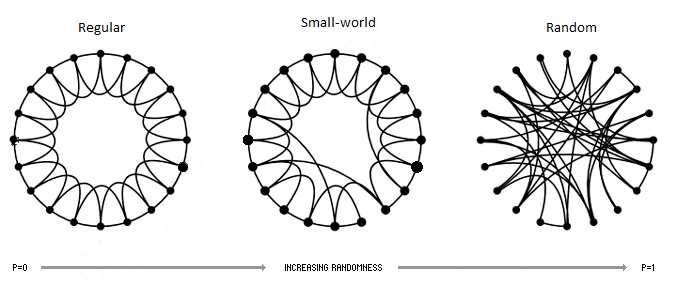
\includegraphics[width=0.7\linewidth]{imagens/watts-sm}
 	\end{center}
 	\small{Fonte: \citet{watts1998collective}.}
 	\label{fig:watts-sm}
 \end{figure} 
 
 As redes \textit{small-worlds} são caracterizadas com duas principais medidas: O tamanho do caminho $L(p)$ e o coeficiente de agrupamento ou coeficiente de aglomeração $C(p)$. $L(p)$ é medido como a média do caminho mais curto de todos pares de vértices \cite{lopes2011redes}. O coeficiente de aglomeração será melhor definido na seção \ref{subsec:coeficienteaglomeracao}.
 
 \subsection{Redes Livres de Escala}
 As redes livres de escala, foram propostas por \citet{barabasi1999emergence}, nelas um nó tem a probabilidade \(P(k)\) de possuir \(k\) arestas obedecendo a lei da potência \(P(k) \sim k^{-\gamma}\), onde $\gamma$ determina o decaimento exponencial  \cite{Albert2002,Antiqueira2005, lopes2011redes}. Segundo \citet{Viana2007} nas redes livres de escala muitos nós tem poucas arestas e poucos nós se ligam a muitos.
 
\citet{lopes2011redes} ainda diz: "Este modelo é baseado em duas regras: crescimento e preferência linear de ligação. A geração de redes Barabási e Albert é iniciada com a inclusão de $n_0 < n$ vértices conectados aleatoriamente". Na etapa de crescimento da rede, a cada instante de tempo $t$ um novo vértice $v$ é adicionado na rede, o número de arestas desse vértice segue uma preferencia linear de ligação da fórmula:
\[ P(v_i \leftrightarrow v_j) = \frac{k_j}{\sum_u k_U}, \forall v_u \in V \]

Sendo $P$ a probabilidade de um vértice $v_i$ ser conectado ao novo vértice $v_j$ é linearmente proporcional ao grau $k_j$ do vértice $v_j$.

{\Huge ainda vou escrever sobre a variação sobre o tempo}
 
     
\subsection{Redes Aleatórias}
Segundo \citet{Viana2007} as redes aleatórias são um sistema formado por $E$ arestas e $N$ vértices, onde as arestas são distribuídas aleatoriamente. 
{\Huge VOU CONTINUAR}
 
\subsection{Coeficiente de Aglomeração}
\label{subsec:coeficienteaglomeracao}
Segundo \citet{Viana2007} o coeficiente de aglomeração mede o quão conectado estão os nós da rede ou do grafo. \citet{Antiqueira2005}  define o coeficiente de aglomeração sendo:\[CA_i = \frac{E_i}{k_i(k_i-1)}\]

\citet{Antiqueira2005}  continua: “Sendo para cada vértice \(i\) existe \(k_i\) arestas, que os ligam a outros \(k_i\) vértices. Se esses \(k_i\) vértices estivessem ligados diretamente à todos os outros vértices do conjunto, haveriam \(k_i(k_i- 1)\) arestas entre eles. E assumindo \(E_i\) o número de arestas que existentes entre os \(k_i\) vértices.	O coeficiente da rede inteira é a média de todos \(CA_i\)”.

\begin{figure}[!h] \centering
	\centering
	\caption{Coeficiente de aglomeração.}
	\subfloat[]{
		\begin{tikzpicture}
		\begin{scope}[xshift=4cm]
		\node[targetnode] (1) {$1$};
		\node[main node] (2) [above right = 2cm  of 1] {$2$};
		\node[main node] (3) [below right = 2cm  of 1] {$3$};
		\node[main node] (4) [right = 2cm  of 2] {$4$};
		\node[main node] (5) [right = 2cm  of 3] {$5$};
		
		\path[draw,thick]
		(1) edge node {} (2)
		(1) edge node {} (3)
		(1) edge node {} (4)
		(1) edge node {} (5)	
		(2) edge node {} (3)
		(2) edge node {} (4)
		(2) edge node {} (5)
		(3) edge node {} (4)
		(3) edge node {} (5)
		(4) edge node {} (5)
		;
		\end{scope}
		\end{tikzpicture}
		\label{fig:grafo-aglomeracao1}
	}
	\subfloat[]{
		\begin{tikzpicture}
		\begin{scope}[xshift=4cm]
		\node[targetnode] (1) {$1$};
		\node[main node] (2) [above right = 2cm  of 1] {$2$};
		\node[main node] (3) [below right = 2cm  of 1] {$3$};
		\node[main node] (4) [right = 2cm  of 2] {$4$};
		\node[main node] (5) [right = 2cm  of 3] {$5$};
		
		\path[draw,thick]
		(1) edge node {} (2)
		(1) edge node {} (3)
		(1) edge node {} (4)
		(1) edge node {} (5)
		(2) edge node {} (4)
		(3) edge node {} (5)
		(4) edge node {} (5)
		;
		\end{scope}
		\end{tikzpicture}
		\label{fig:grafo-aglomeracao2}
	}
	\
	\small{\leftline{Fonte: Autor.}}
	\label{fig:grafo-aglomeracao}
\end{figure}

Na Figura \ref{fig:grafo-aglomeracao1}, assumindo o peso de todas as arestas como 1, o coeficiente de aglomeração do vértice em azul é 1, já na Figura \ref{fig:grafo-aglomeracao2} o coeficiente do vértice em azul segundo a fórmula é $\frac{1}{2}$. 
    


\section{\textit{League of Legends}}
\label{chap:lol}
O jogo \textit{League of Legends} é um jogo classificado como arena de batalha online de multi jogadores (do inglês \textit{Multiplayer Online Battle Arena} ) ou conhecido também como MOBA, que é um estilo de jogo onde duas equipes se enfrentam em um campo de batalha e cada jogador controla o seu personagem, mais chamado de herói ou campeão. O objetivo do MOBA é derrotar a equipe adversária destruindo a construção principal da equipe inimiga.

	A arena onde acontece o jogo é uma arena onde normalmente o mapa inicialmente é  espelhado,  ou  seja, o lado que cada time está não  oferece vantagens  exclusivas.  O mapa é composto  de  três caminhos até a base inimiga.
    
%%preciso conferir se essa foto é acervo, ou é do lol

\begin{figure}[H]
	\caption{Mapa do jogo de \textit{League of Legends}}
	\begin{center}
		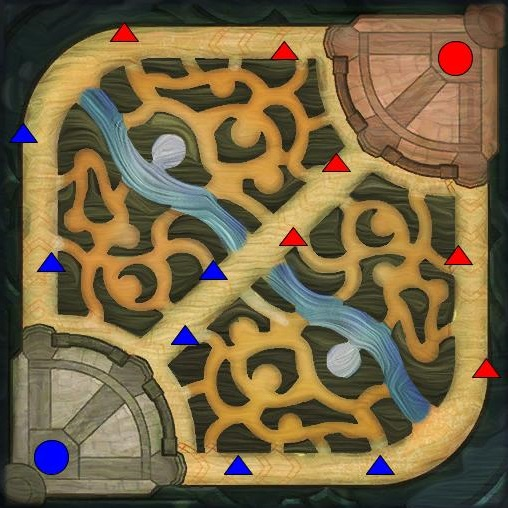
\includegraphics{imagens/mapa_lol.jpg}
	\end{center}
	\small{Fonte: Autor (2018).}
	\label{fig:mapa_lol}
\end{figure}

	A Figura \ref{fig:mapa_lol} mostra como é realmente o mapa do jogo, sendo que os círculos mostram a localização da construção principal, e os triângulos as construções de suporte de cada equipe, sendo azul uma equipe e vermelho a outra.
    
	Com o início do jogo cada jogador escolhe  um  herói  diferente, onde  cada  herói tem um conjunto de características únicas, como habilidades especiais,  seu impacto  no jogo,  na equipe adversária e na equipe aliada.
    
	Depois de escolher os heróis de cada equipe, cada jogador deve procurar adquirir recursos no jogo e objetivos para conseguir vantagens. Os recursos são limitados por equipe e por tempo, ou seja, deve ser bem escolhido quem ficará com a maior parte dos recursos da equipe.

\section{Estado da Arte}


{\Huge VOU REFAZER}
